\documentclass[aspectratio=169,11pt]{beamer}
\def\courseweek{2}
% Shared style for the Introduction to Information Geometry lecture slides.
% Compile the lecture .tex files from this directory.
\providecommand{\courseweek}{1}
\usepackage[T1]{fontenc}
\usepackage[utf8]{inputenc}
\usepackage[sc]{mathpazo}
\renewcommand{\sfdefault}{lmss}
\renewcommand{\ttdefault}{lmtt}
\usepackage{amsmath,amssymb,mathtools}
\usepackage{tikz}
\usetikzlibrary{arrows.meta,calc,positioning}
\usepackage{pgfplots}
\pgfplotsset{compat=1.18}
\usepackage{booktabs}

\definecolor{courseink}{HTML}{173749}
\definecolor{coursemuted}{HTML}{526674}
\definecolor{courseteal}{HTML}{0E7287}
\definecolor{coursecopper}{HTML}{B66B43}
\definecolor{courseline}{HTML}{D4E0E3}
\definecolor{coursepale}{HTML}{EFF5F5}

\setbeamercolor{normal text}{fg=courseink,bg=white}
\setbeamercolor{structure}{fg=courseteal}
\setbeamercolor{frametitle}{fg=courseink,bg=white}
\setbeamercolor{title}{fg=courseink}
\setbeamercolor{subtitle}{fg=coursemuted}
\setbeamercolor{block title}{fg=courseink,bg=white}
\setbeamercolor{block body}{fg=courseink,bg=white}
\setbeamercolor{alerted text}{fg=coursecopper}
\setbeamerfont{title}{family=\rmfamily,series=\bfseries,size=\fontsize{32}{37}}
\setbeamerfont{frametitle}{family=\rmfamily,series=\bfseries,size=\fontsize{26}{31}}
\setbeamerfont{normal text}{size=\fontsize{18}{22}}
\setbeamerfont{subtitle}{size=\fontsize{17}{21}}
\setbeamersize{text margin left=0.78cm,text margin right=0.78cm}
\setbeamertemplate{navigation symbols}{}
\setbeamertemplate{itemize items}[circle]
\setbeamertemplate{enumerate items}[default]
\setbeamertemplate{blocks}[default]
\setlength{\parskip}{0.22em}
\setbeamertemplate{footline}{%
  \leavevmode\hbox to \paperwidth{\hspace{.78cm}%
  {\color{coursemuted}\fontsize{8.5}{10}\selectfont Introduction to Information Geometry \hspace{.32cm} / \hspace{.32cm} Week \courseweek}%
  \hfill{\color{coursemuted}\fontsize{8.5}{10}\selectfont \insertframenumber\hspace{.17cm}/\hspace{.17cm}\inserttotalframenumber}\hspace{.78cm}}%
  \vskip.17cm
}
\setbeamertemplate{frametitle}{%
  \vspace{.13cm}
  \insertframetitle\par
  \vspace{.08cm}
}
\setbeamertemplate{title page}{%
  \vspace*{1.00cm}
  {\color{courseteal}\fontsize{10}{13}\selectfont\bfseries
  INTRODUCTION TO INFORMATION GEOMETRY\par}
  \vspace{.40cm}
  {\usebeamerfont{title}\usebeamercolor[fg]{title}\inserttitle\par}
  \vspace{.22cm}
  {\usebeamerfont{subtitle}\usebeamercolor[fg]{subtitle}\insertsubtitle\par}
  \vfill
  {\color{coursemuted}\fontsize{13}{16}\selectfont Christopher Lee\par}
  \vspace{.34cm}
}

\pgfplotsset{
  courseplot/.style={
    width=11.05cm,
    height=5.15cm,
    axis line style={coursemuted!75},
    tick style={coursemuted!65},
    ticklabel style={font=\scriptsize,color=coursemuted},
    label style={font=\normalsize,color=courseink},
    grid=major,
    major grid style={courseline!70,line width=.4pt},
    line width=1.45pt,
    legend style={font=\small,draw=none,fill=none,at={(.98,.03)},anchor=south east},
    clip=true
  }
}

\newcommand{\highlightmath}[1]{{\color{courseteal}#1}}
\newcommand{\thinrule}{\par\vspace{.25cm}{\color{courseline}\rule{\linewidth}{.8pt}}\par}

% A one-dimensional state space.  x=0 and x=1 are placed at 0 and 9 units.
\newcommand{\stateinterval}[1]{%
 \begin{tikzpicture}[x=1cm,y=1cm]
   \draw[courseink,line width=1.25pt] (0,0)--(9,0);
   \foreach \pos/\lab in {0/0,9/1} {
     \fill[courseink] (\pos,0) circle(2.7pt);
     \node[below=9pt,text=coursemuted] at (\pos,0) {\(\lab\)};
   }
   #1
 \end{tikzpicture}%
}

% Paired pages are separate frames in the PDF, with matching titles.
% Supply the whole frame body for each version; the instructor may edit them
% independently without changing overlay logic.
\newcommand{\coursepair}[3]{%
  \begin{frame}{#1}#2\end{frame}%
  \begin{frame}{#1}#3\end{frame}%
}

% Equilateral representation of the categorical simplex, in barycentric
% coordinates with vertices A=(0,0), B=(1,0), C=(1/2,sqrt(3)/2).
\newcommand{\coursesimplex}[1]{%
 \begin{tikzpicture}[scale=4.9]
  \fill[coursepale] (0,0)--(1,0)--(.5,.8660254)--cycle;
  \draw[courseink,line width=.65pt] (0,0)--(1,0)--(.5,.8660254)--cycle;
  \node[below left,font=\small] at (0,0) {A};
  \node[below right,font=\small] at (1,0) {B};
  \node[above,font=\small] at (.5,.8660254) {C};
  #1
 \end{tikzpicture}%
}

\title{Payoff Matrices and Expected Fitness}
\subtitle{Week 2 \(\cdot\) Lecture 1}
\date{}
\begin{document}

\begin{frame}[plain]\titlepage\end{frame}

\begin{frame}{Fitness comes from encounters}
In a well-mixed population, a type meets A with probability \(x\)
and B with probability \(1-x\).
\vspace{.38cm}
\[
\highlightmath{M=\begin{pmatrix}a&b\\c&d\end{pmatrix}}
\]
\vspace{.37cm}
\begin{center}
\begin{tabular}{@{}lcc@{}}
 & Opponent A & Opponent B\\\midrule
Type A receives & \(a\) & \(b\)\\
Type B receives & \(c\) & \(d\)
\end{tabular}
\end{center}
\end{frame}

\begin{frame}{A weighted average of encounters}
An A individual receives payoff \(a\) from an A opponent
and payoff \(b\) from a B opponent.
\vspace{.4cm}
\[
\highlightmath{f_A(x)=ax+b(1-x)}.
\]
\vspace{.55cm}
Similarly,
\[
\highlightmath{f_B(x)=cx+d(1-x)}.
\]
\vspace{.35cm}
Both expected fitnesses depend on the current population composition.
\end{frame}

\coursepair{A matrix becomes a dynamical model}{
Let \(M=\begin{pmatrix}2&4\\3&1\end{pmatrix}\).
\vspace{.35cm}
\[
f_A(x)=2x+4(1-x)=\;?,
\qquad f_B(x)=3x+(1-x)=\;?.
\]
\vspace{.45cm}
Find the fitnesses at \(x=\frac14\).
\[
f_A(\tfrac14)=\;?,\qquad f_B(\tfrac14)=\;?.
\]
}{
Let \(M=\begin{pmatrix}2&4\\3&1\end{pmatrix}\).
\vspace{.35cm}
\[
f_A(x)=2x+4(1-x)=\highlightmath{4-2x},
\qquad f_B(x)=3x+(1-x)=\highlightmath{1+2x}.
\]
\vspace{.45cm}
At \(x=\frac14\),
\[
f_A(\tfrac14)=\highlightmath{\tfrac72},\qquad
f_B(\tfrac14)=\highlightmath{\tfrac32}.
\]
}

\begin{frame}{The two expected fitness functions}
\vspace{-.25cm}
\begin{center}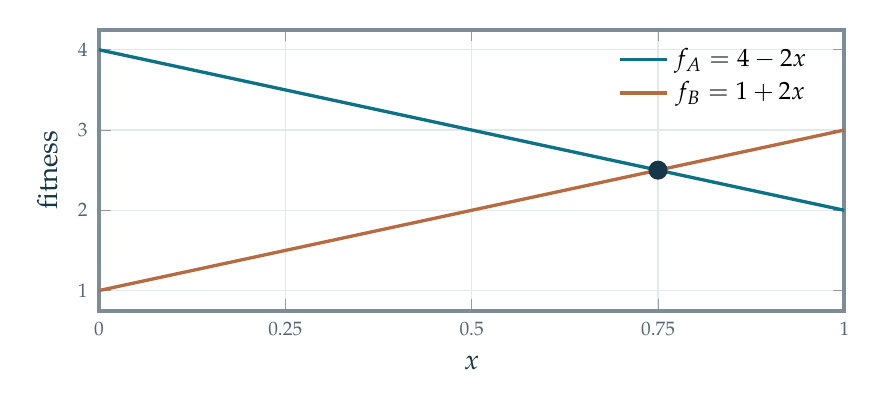
\begin{tikzpicture}
\begin{axis}[courseplot,xmin=0,xmax=1,ymin=.75,ymax=4.25,
 xlabel={$x$},ylabel={fitness},xtick={0,.25,.5,.75,1},ytick={1,2,3,4},
 legend style={at={(.97,.98)},anchor=north east}]
\addplot[courseteal,very thick,domain=0:1]{4-2*x};\addlegendentry{\(f_A=4-2x\)}
\addplot[coursecopper,very thick,domain=0:1]{1+2*x};\addlegendentry{\(f_B=1+2x\)}
\addplot[only marks,courseink,mark=*,mark size=2.7pt] coordinates {(.75,2.5)};
\end{axis}\end{tikzpicture}\end{center}
\vspace{-.15cm}
Where the two lines intersect, both types have equal fitness.
\end{frame}

\begin{frame}{The advantage is an affine function}
Subtract the fitnesses:
\vspace{.4cm}
\[
\highlightmath{\Delta(x)=f_A(x)-f_B(x)}
\]
\vspace{.28cm}
\[
=\underbrace{(b-d)}_{\Delta(0)}+
\underbrace{(a-b-c+d)}_{\text{slope}}x.
\]
\vspace{.52cm}
The differential equation is
\[
\highlightmath{x'=x(1-x)\Delta(x)}.
\]
\end{frame}

\begin{frame}{Reading the advantage at the endpoints}
\[
\Delta(0)=b-d, \qquad \Delta(1)=a-c.
\]
\vspace{.5cm}
\begin{itemize}\setlength{\itemsep}{.47cm}
\item At \(x\approx0\), a rare A mostly meets B. A increases when \(b>d\).
\item At \(x\approx1\), a rare B mostly meets A. B increases when \(c>a\).
\end{itemize}
\vspace{.38cm}
These invasion tests determine the direction of motion near the two ends.
\end{frame}

\begin{frame}{Four phase portraits from two signs}
\begin{center}
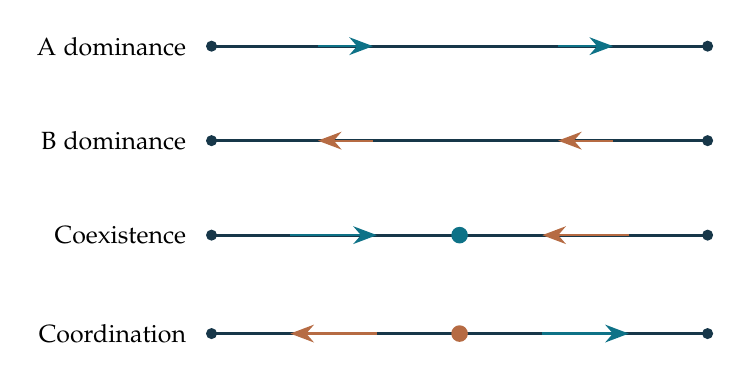
\begin{tikzpicture}[x=1cm,y=1cm]
\foreach \y/\name in {2.65/{A dominance},1.45/{B dominance},.25/{Coexistence},-1.0/{Coordination}}{
 \node[anchor=east,font=\small] at (-.2,\y){\name};
 \draw[courseink,line width=1.1pt] (0,\y)--(6.3,\y);
 \fill[courseink] (0,\y) circle(2pt);\fill[courseink] (6.3,\y) circle(2pt);
}
\foreach \x in {1.35,4.4}{\draw[-{Stealth[length=3mm]},courseteal,thick](\x,2.65)--++(.7,0);\draw[-{Stealth[length=3mm]},coursecopper,thick](\x+.7,1.45)--++(-.7,0);}
\draw[-{Stealth[length=3mm]},courseteal,thick](1,.25)--(2.1,.25);
\draw[-{Stealth[length=3mm]},coursecopper,thick](5.3,.25)--(4.2,.25);
\fill[courseteal] (3.15,.25) circle(3pt);
\draw[-{Stealth[length=3mm]},coursecopper,thick](2.1,-1)--(1,-1);
\draw[-{Stealth[length=3mm]},courseteal,thick](4.2,-1)--(5.3,-1);
\fill[coursecopper] (3.15,-1) circle(3pt);
\end{tikzpicture}
\end{center}
\vspace{.08cm}
\centering The signs of \(\Delta(0)\) and \(\Delta(1)\) determine the case.
\end{frame}

\coursepair{A coordination example}{
Consider \(M=\begin{pmatrix}4&1\\2&3\end{pmatrix}\).
\vspace{.37cm}
Find \(\Delta(0)\), \(\Delta(1)\), and the interior equilibrium.
\vspace{.35cm}
\[
\Delta(0)=\;?,\qquad \Delta(1)=\;?,\qquad x^*=\;?.
\]
\vspace{.4cm}
Which endpoint does a solution approach from \(x(0)=0.35\)?
}{
Consider \(M=\begin{pmatrix}4&1\\2&3\end{pmatrix}\).
\vspace{.37cm}
The advantage is \(\Delta(x)=\highlightmath{4x-2}\).
\vspace{.35cm}
\[
\Delta(0)=\highlightmath{-2},\quad\Delta(1)=\highlightmath{2},
\quad x^*=\highlightmath{\tfrac12}.
\]
\vspace{.4cm}
The solution from \(x(0)=0.35\) approaches \(0\).
}

\coursepair{The coordination phase line}{
For \(x'=x(1-x)(4x-2)\), the interior equilibrium is \(x^*=\frac12\).
\vspace{.6cm}
\begin{center}\stateinterval{\fill[coursecopper](4.5,0)circle(4pt);\node[above=10pt]at(4.5,0){\(\frac12\)};}\end{center}
\vspace{.45cm}
Draw the arrows. Determine the basins of attraction.
}{
For \(x'=x(1-x)(4x-2)\), the interior equilibrium is \(x^*=\frac12\).
\vspace{.6cm}
\begin{center}\stateinterval{
\fill[coursecopper](4.5,0)circle(4pt);\node[above=10pt]at(4.5,0){\(\frac12\)};
\draw[-{Stealth[length=4mm]},courseteal,very thick](3.2,0)--(1.4,0);
\draw[-{Stealth[length=4mm]},courseteal,very thick](5.8,0)--(7.6,0);
}\end{center}
\vspace{.45cm}
The basins are \(\highlightmath{[0,\frac12)}\) and \(\highlightmath{(\frac12,1]}\).
}

\begin{frame}{The one-dimensional conclusion}
For a two-strategy payoff matrix,
\[
x'=x(1-x)\big[(b-d)+(a-b-c+d)x\big].
\]
\vspace{.55cm}
The difference between the rows determines the motion.
\vspace{.40cm}
\begin{itemize}\setlength{\itemsep}{.35cm}
\item Its values at \(0\) and \(1\) determine the phase portrait.
\item Its zero, when interior, locates the coexistence or threshold state.
\end{itemize}
\end{frame}

\end{document}
